% =====================================================================
%  draft.tex
%  "What Does the Frechet Music Distance Measure? A Sensitivity Study
%   of Tokenization and Embedding Choices for Symbolic Music"
%
%  Self-contained: compile with `pdflatex draft.tex` (run twice for refs).
%  The only external assets are the figures in
%  results/plots/sensitivity_pivot/paper/ (see \graphicspath below) --
%  compile from the repository root, or copy that folder next to this file.
%
%  All tables/figures were generated from the result CSVs by
%  scripts/generate_draft_tables.py and scripts/generate_draft_figures.py
%  (no number was typed by hand); the tables are inlined below.
% =====================================================================
\documentclass[11pt]{article}

\usepackage[utf8]{inputenc}
\usepackage[T1]{fontenc}
\usepackage[a4paper,margin=2.4cm]{geometry}
\usepackage{amsmath,amssymb}
\usepackage{graphicx}
\usepackage{booktabs}
\usepackage{array}
\usepackage{caption}
\usepackage{xcolor}
\usepackage{microtype}
\usepackage[hidelinks]{hyperref}

\newcommand{\snr}{\mathrm{SNR}}
\newcommand{\fmd}{\mathrm{FMD}}
\graphicspath{{results/plots/sensitivity_pivot/paper/}}
\captionsetup{font=small,labelfont=bf}

\title{\textbf{What Does the Fr\'echet Music Distance Measure?\\
A Sensitivity Study of Tokenization and Embedding Choices\\
for Symbolic Music}}

\author{Micha{\l} Fereniec \quad Bartosz S\k{e}dzikowski\\[2pt]
\small Warsaw University of Technology, Faculty of Electronics and Information Technology\\
\small Course: WIMU (Music Information Retrieval) \quad Supervisor: mgr in\.z.\ Tomasz Radzikowski}

\date{June 2026}

\begin{document}
\maketitle

\begin{abstract}
The Fr\'echet Music Distance (FMD) is increasingly used to evaluate
generative symbolic-music systems, but an FMD score is not a property of
the music alone: it is produced by a \emph{pipeline} --- an input
representation, a pre-trained embedding model, and the Fr\'echet formula
--- and different pipelines measure different things. We profile five FMD
configurations --- four primary pipelines spanning two embedding models
(MusicBERT, CLaMP-1/2) and three input representations (MidiTok REMI/TSD
token streams, MIDI-text format, ABC notation), plus a same-model control
that disentangles the representation from the model --- over six datasets
and five controlled, musically interpretable perturbations of MIDI. Our central
methodological point is that \emph{raw FMD is not comparable across
embedding spaces}: CLaMP embeddings are $L_2$-normalised (unit sphere,
small FMD) whereas MusicBERT's are not (large FMD), so the configurations'
noise floors differ by roughly $60\times$ for purely geometric reasons.
We therefore compare configurations only through scale-invariant
quantities: a per-configuration signal-to-noise ratio (SNR), permutation
and per-file Wilcoxon tests, and Spearman rank agreement. Three findings
emerge.
(i)~Removing note velocity is the only perturbation that moves the
embedding distribution above the sampling-noise floor, and only in
representations that encode velocity (SNR $1.2$--$4.2$, permutation
$p\le0.02$, for REMI/TSD/MTF); under ABC, which has no velocity channel,
the perturbed rendering is character-identical and FMD is exactly zero.
The same-model control makes this causal: CLaMP-2 detects velocity under
MTF and is structurally blind under ABC. A per-file paired analysis with a
re-encoding noise floor (Wilcoxon, Holm-corrected) and a full replication
on a second corpus confirm the profile; microtiming and tempo stay at or
below the detection floor everywhere.
(ii)~Yet across $15$ dataset pairs all five pipelines rank corpora largely
alike (Spearman $\rho=0.51$--$0.91$; MTF vs.\ ABC $\rho=0.907$,
$p<0.001$): corpus-level stylistic ranking is carried by the pitch--rhythm
core that every representation shares, and is robust precisely where
attribute-level sensitivity is not.
(iii)~Even the tokenizer alone (REMI vs.\ TSD, same model) reshapes the
sensitivity profile and weakens ranking agreement ($\rho=0.44$, n.s.). We
conclude that the input representation decides which musical attributes
FMD can perceive, give practitioner guidance, and document a cautionary
negative result: naive cross-model FMD comparison is a scale artifact, not
a finding.
\end{abstract}

\noindent\textbf{Keywords:} Fr\'echet Music Distance, symbolic music
evaluation, MIDI tokenization, music embeddings, CLaMP, MusicBERT,
perturbation analysis, sensitivity.

% =====================================================================
\section{Introduction}
% =====================================================================
Distribution-level distances of the Fr\'echet family have become the
default way to judge generative models: the Fr\'echet Inception Distance
(FID) for images~\cite{heusel2017fid} and the Fr\'echet Audio Distance
(FAD) for audio~\cite{kilgour2019fad} compare a reference and a candidate
set by fitting a Gaussian to each in a pre-trained embedding space and
measuring the Fr\'echet (Wasserstein-2) distance between the two
Gaussians~\cite{dowson1982frechet}. The Fr\'echet Music Distance
(FMD)~\cite{retkowski2025fmd} transplants this recipe to \emph{symbolic}
music, replacing the perceptual backbone with a symbolic-music encoder.

This convenience hides a dependency that matters for anyone reporting an
FMD number. An FMD score is produced not by the music alone but by a
\emph{pipeline} with at least three moving parts: (i)~how a MIDI file is
turned into model input (a tokenization such as REMI or TSD, a MIDI-text
rendering, or a score-like ABC transcription); (ii)~which pre-trained
model embeds that input; and (iii)~the Fr\'echet formula itself. Two
pipelines that disagree about which musical attributes survive the
encoding will assign systematically different distances to the
\emph{same} pair of corpora. If the community compares systems by FMD, it
must first understand what each FMD variant is actually sensitive to.

We study this empirically. Rather than proposing a new metric, we treat
existing FMD pipelines as objects of measurement and ask: \emph{given a
fixed configuration, which musical properties does it respond to, and how
does that depend on the tokenizer and the embedding model?} We answer it
with a perturbation protocol --- stripping one expressive attribute
(dynamics, microtiming, tempo) from the data and measuring how far the
embedding distribution moves --- calibrated against each pipeline's own
sampling noise, plus a cross-dataset ranking whose agreement across
pipelines we test with Spearman's $\rho$.

\paragraph{A pivot, and an honest accounting.}
An earlier iteration of this project (a)~pursued a \emph{normalized} FMD
intended to make scores comparable across models, and (b)~included a
configuration nominally labelled ``CLaMP-2 + REMI'' that in fact fed the
model ABC notation. We retired both. CLaMP does not natively consume
MidiTok token streams, so token-based representations here are routed to
MusicBERT~\cite{zeng2021musicbert} --- a model designed for symbolic-music
tokens --- while CLaMP receives only its native MIDI-text and ABC inputs.
And the cross-model FMD gap we had hoped to ``normalize away'' turns out to
be a property of embedding geometry (\S\ref{sec:background}), not of the
music; the constructive replacement is to compare each pipeline
\emph{against itself} and to compare pipelines only through scale-invariant
statistics.

\paragraph{Contributions.}
\begin{enumerate}\itemsep2pt
  \item A perturbation-based \emph{sensitivity-profiling} protocol for FMD
  pipelines, using musically interpretable, reversible ablations of MIDI,
  with each effect calibrated by a per-configuration noise floor into a
  dimensionless, cross-pipeline-comparable SNR and tested with a two-sample
  permutation test (\S\ref{sec:method}).
  \item Causal evidence that the input representation, not the model, gates
  what FMD detects: a same-model control (CLaMP-2 fed MTF vs.\ ABC) shows
  the velocity response appearing and vanishing with the representation
  alone, and the full sensitivity profile replicates on a second corpus;
  microtiming and tempo are below the noise floor for all configurations
  (\S\ref{sec:results}).
  \item A scale-invariant cross-configuration analysis over $15$ dataset
  pairs showing that corpus-level stylistic ranking is largely robust to
  the pipeline ($\rho=0.51$--$0.91$ across all five configurations; MTF
  vs.\ ABC $\rho=0.907$) even though attribute-level sensitivity is not ---
  the two questions ``does FMD rank corpora sensibly?'' and ``does FMD see
  attribute X?'' have different answers (\S\ref{sec:results}).
  \item A documented negative result and a caution for the field: comparing
  raw FMD across embedding models is a scale artifact
  (\S\ref{sec:background},~\S\ref{sec:discussion}), with practitioner
  guidance.
\end{enumerate}

% =====================================================================
\section{Related Work}
% =====================================================================
\paragraph{Fr\'echet distances for generative evaluation.}
FID~\cite{heusel2017fid} popularised fitting Gaussians in a pre-trained
feature space and using the closed-form Fr\'echet distance between
Gaussians~\cite{dowson1982frechet}; FAD~\cite{kilgour2019fad} adapted it to
audio. FMD~\cite{retkowski2025fmd} brings the construction to symbolic
music and is the metric we profile. A recurring concern for the whole
family is estimator bias and instability when the number of samples is
small relative to the embedding dimension, which inflates the covariance
term --- a regime we operate in and quantify.

\paragraph{Symbolic-music embeddings.}
MusicBERT~\cite{zeng2021musicbert} pre-trains a Transformer on symbolic
music with an OctupleMIDI encoding for music-understanding tasks.
CLaMP~\cite{wu2023clamp} learns a contrastive language--music space over
ABC notation, and CLaMP-2~\cite{wu2024clamp2} extends this to a multimodal
setting with an M3 patch encoder operating on a MIDI-text format (MTF).
Crucially for our analysis, the contrastive CLaMP models $L_2$-normalise
their output embeddings (they are trained with cosine similarity), whereas
MusicBERT exposes raw hidden states; this geometric difference, not any
musical one, dominates the raw FMD scale.

\paragraph{MIDI tokenization.}
MidiTok~\cite{fradet2021miditok} provides interchangeable tokenizations of
MIDI, including REMI~\cite{huang2020remi} and TSD. The tokenizer decides
which attributes (velocity bins, time-shifts, tempo events) are even
representable downstream, and is therefore a first-class variable in any
FMD pipeline; Le et al.~\cite{le2024nlpsurvey} survey NLP methods for
symbolic music and motivate treating tokenization as a consequential
modelling decision rather than preprocessing.

\paragraph{Gap.}
Prior work introduces these metrics, models, and tokenizers, but does not
systematically characterise \emph{what an FMD pipeline becomes blind or
sensitive to as a function of those choices}, nor caution against comparing
raw FMD across embedding spaces. We address both.

% =====================================================================
\section{Background: the Fr\'echet Music Distance}
\label{sec:background}
% =====================================================================
Given two embedding sets with empirical means $\mu_1,\mu_2$ and covariances
$\Sigma_1,\Sigma_2$, FMD is the squared Fr\'echet distance between the
fitted Gaussians:
\begin{equation}
\fmd = \lVert \mu_1-\mu_2\rVert_2^2 \;+\;
\operatorname{Tr}\!\Big(\Sigma_1+\Sigma_2-2(\Sigma_1\Sigma_2)^{1/2}\Big).
\label{eq:fmd}
\end{equation}
We regularise covariances with a small ridge ($\varepsilon=10^{-4}$ on the
diagonal) and fall back to an eigenvalue evaluation of
$\operatorname{Tr}(\Sigma_1\Sigma_2)^{1/2}=\sum_i\sqrt{\lambda_i}$ when the
matrix square root returns non-negligible imaginary parts.

Equation~\eqref{eq:fmd} is \emph{not scale-free}. If one model emits
unit-norm vectors while another emits vectors of norm $\sim\!15$, both the
mean term and the trace term scale with the geometry of the
space.\footnote{Concretely, scaling all embeddings of a configuration by a
constant $c$ multiplies $\fmd$ by $c^2$; an $L_2$-normalised space ($\lVert
e\rVert=1$) and an unnormalised one are related by exactly such a (here,
non-constant but systematically large) factor.} Consequently the
\emph{magnitude} of an FMD score carries information about the embedding
space at least as much as about the music. This is the formal reason
cross-model comparison of raw FMD is unsound, and the motivation for the
scale-invariant analyses of \S\ref{sec:method}.

% =====================================================================
\section{Methodology}
\label{sec:method}
% =====================================================================

\subsection{Configurations}
We evaluate four primary pipelines plus one control
(Table~\ref{tab:configs}), chosen so that pairs differ in exactly one
factor. \texttt{MusicBERT-REMI} and \texttt{MusicBERT-TSD} share a model
and differ only in the MidiTok tokenizer, isolating \emph{tokenization}.
\texttt{CLaMP2-MTF} and \texttt{CLaMP1-ABC} change both the model and its
native representation; to disentangle the two we add the control
configuration \texttt{CLaMP2-ABC} --- the \emph{same} model as
\texttt{CLaMP2-MTF} fed the \emph{same} ABC representation as
\texttt{CLaMP1-ABC}. This is a legitimate input, not an off-distribution
trick: CLaMP-2's M3 music encoder is trained on both ABC notation and
MTF~\cite{wu2024clamp2}. Within CLaMP-2, MTF vs.\ ABC then isolates the
\emph{representation}; within ABC, CLaMP-2 vs.\ CLaMP-1 isolates the
\emph{model}. All models emit $768$-dimensional embeddings, so
Equation~\eqref{eq:fmd} is dimensionally identical across them; only the
geometry differs.

\begin{table}[t]
\centering
\caption{FMD configurations. ABC notation has no velocity channel by
construction; CLaMP embeddings are $L_2$-normalised, MusicBERT's are not.
\texttt{CLaMP2-ABC} is the same-model control that separates the
representation effect from the model effect.}
\label{tab:configs}
\small
\begin{tabular}{@{}lllc@{}}
\toprule
Config & Model & Input & Norm. \\
\midrule
\texttt{MusicBERT-REMI} & MusicBERT & REMI tokens (MidiTok) & no \\
\texttt{MusicBERT-TSD}  & MusicBERT & TSD tokens (MidiTok)  & no \\
\texttt{CLaMP2-MTF}     & CLaMP-2   & MIDI-text format      & yes \\
\texttt{CLaMP1-ABC}     & CLaMP-1   & ABC notation          & yes \\
\texttt{CLaMP2-ABC} (control) & CLaMP-2 & ABC notation      & yes \\
\bottomrule
\end{tabular}
\end{table}

We use the released checkpoints (\texttt{manoskary/musicbert},
\texttt{sander-wood/clamp2}, \texttt{clamp-small-512}). For CLaMP, MTF is
rendered from raw MIDI via \texttt{mido}, and ABC by our own deterministic
renderer --- pitch, rhythm (sixteenth-note grid, \texttt{L:1/16}), meter,
and the global tempo marking, with no velocity channel, exactly as in the
ABC standard; both are bar-patched by the M3 character
patcher.\footnote{We render ABC ourselves because \texttt{music21} offers
no ABC \emph{export}: its \texttt{write('abc')} silently emits the object
repr rather than notation. An earlier iteration of this study was affected,
which the per-file retest analysis of \S\ref{sec:method} exposed
immediately --- one practical argument for building such checks into
evaluation pipelines. The M3 patcher additionally requires
\texttt{unidecode}.} For MusicBERT, a MidiTok token stream is rendered to a
string of token identifiers and encoded, returning the \texttt{[CLS]}
state; we flag this rendering as a limitation (\S\ref{sec:limitations}).

\subsection{Datasets and perturbations}
We use six datasets: \textbf{MAESTRO}~\cite{hawthorne2019maestro}
(expressive classical piano), \textbf{POP909}~\cite{wang2020pop909}, and
four Lakh-derived genre subsets (\emph{classical, jazz, rock, rap}); $80$
files each, fixed seed. This yields $\binom{6}{2}=15$ dataset pairs, above
the $n\ge 10$ threshold at which the rank-agreement statistic below is
reported as interpretable. The perturbation study runs on MAESTRO, which is
rich in the attributes we ablate, and is replicated on POP909 to check that
the sensitivity profile is not an artifact of one corpus.

Each perturbation removes one expressive attribute while leaving pitch and
note structure intact: \emph{velocity flattening} (all velocities $\to64$),
\emph{time quantization} (onsets/durations to a $16$th-note grid),
\emph{tempo flattening} ($\to120$\,BPM), and \emph{all combined}.

\subsection{Scale-invariant analyses}
Because raw FMD is not comparable across configurations
(\S\ref{sec:background}), every cross-configuration quantity we report is
scale-invariant.

\paragraph{Noise floor and SNR.}
For configuration $c$ on a dataset we randomly split the files into halves
$A,B$ and define the noise floor $\eta_c=\fmd_c(A,B)$ (a stable pipeline
gives $\eta_c\!\approx\!0$). For perturbation $p$ we report the
dimensionless ratio
\begin{equation}
\snr_c(p)=\frac{\fmd_c(\text{original},\,\text{perturbed}_p)}{\eta_c},
\label{eq:snr}
\end{equation}
whose denominator absorbs the geometric scale of the embedding space.
$\snr_c(p)\ge 1$ means the perturbation moves the distribution more than
within-dataset resampling does.

\paragraph{Permutation significance.}
To test whether a perturbation has \emph{any} systematic effect we use a
two-sample permutation test: pool the original and perturbed embeddings,
randomly relabel them into two groups of the original sizes, recompute FMD,
and repeat ($200$ permutations); the $p$-value is the fraction of permuted
FMDs at least as large as the observed one.\footnote{The permutation test
is matched in sample size ($80$ vs.\ $80$) and free of the upward tie-bias
of bootstrap resampling, so it is the appropriate significance test here;
the split-half floor of Eq.~\eqref{eq:snr} is retained only as the
effect-size scale.} We call an attribute \emph{detected} when it is
permutation-significant ($p<0.05$) \emph{and} exceeds the noise floor
($\snr\ge1$). A bootstrap ($100$ resamples) gives the FMD confidence
interval.

\paragraph{Per-file paired analysis with a retest floor.}
FMD is a distribution-level statistic; to show that its signal is not an
artifact of fitting Gaussians at $n\ll d$, we add a sample-level view. For
every file we measure the cosine distance between its original and
perturbed embedding (cosine, being norm-free, is meaningful in every
configuration), yielding $N$ paired observations per configuration and
perturbation. Each file is also encoded a \emph{second} time without any
perturbation; this \emph{retest} distance is the per-file encoding-noise
floor, and a perturbation counts as a file-level effect only if it moves
the embedding more than re-encoding the same unperturbed file does
(one-sided Wilcoxon signed-rank, Holm-corrected per corpus). Files are
aligned across conditions, and the same-model control contrast compares
retest-corrected velocity shifts under MTF vs.\ ABC within CLaMP-2 ---
embeddings of the same model, hence the same space, so no cross-space
caveat applies.

\paragraph{Rank agreement.}
For each configuration we rank the $15$ dataset pairs by FMD and compute
Spearman's $\rho$ between configurations. Because $\rho$ depends only on
rank order it is invariant to the embedding scale, making it a sound way to
ask whether two pipelines order corpora the same way despite incomparable
magnitudes. Finally, a bootstrap ($50$ resamples, $N=80$) of the
MAESTRO--POP909 distance gives the scale-invariant coefficient of variation
$\mathrm{CV}=\sigma/\mu$.

% =====================================================================
\section{Results}
\label{sec:results}
% =====================================================================

\subsection{Noise floors differ by orders of magnitude for geometric reasons}
Table~\ref{tab:selfsim} reports split-half FMD. The CLaMP configurations
sit near $0.02$--$0.18$; the MusicBERT configurations near $1.2$--$2.3$.
This gap of one to two orders of magnitude is \emph{not} evidence that
CLaMP is correspondingly ``more consistent''; it is the expected
consequence of $L_2$-normalised vs.\ unnormalised embeddings entering the
scale-sensitive Equation~\eqref{eq:fmd} (\S\ref{sec:background}). It is
exactly why a per-pipeline noise floor is required before any
cross-configuration statement. Figure~\ref{fig:floor} shows the same data
on a log axis.

\begin{table}[t]
\centering
\caption{Self-similarity (split-half FMD). Lower is more stable. The
CLaMP/MusicBERT gap is a geometric artifact of embedding normalisation, not
a musical property. Generated from \texttt{self\_similarity.csv}.}
\label{tab:selfsim}
\small
\begin{tabular}{@{}lcccccc@{}}
\toprule
Configuration & classical & jazz & maestro & pop909 & rap & rock \\
\midrule
\texttt{MusicBERT-REMI} & 1.877 & 1.800 & 2.124 & 1.572 & 1.707 & 1.580 \\
\texttt{MusicBERT-TSD} & 1.514 & 1.351 & 2.308 & 2.323 & 1.275 & 1.213 \\
\texttt{CLaMP2-MTF} & 0.027 & 0.021 & 0.036 & 0.029 & 0.020 & 0.023 \\
\texttt{CLaMP1-ABC} & 0.054 & 0.076 & 0.054 & 0.058 & 0.075 & 0.077 \\
\texttt{CLaMP2-ABC} & 0.164 & 0.167 & 0.181 & 0.163 & 0.132 & 0.118 \\
\bottomrule
\end{tabular}
\end{table}

\begin{figure}[t]
\centering
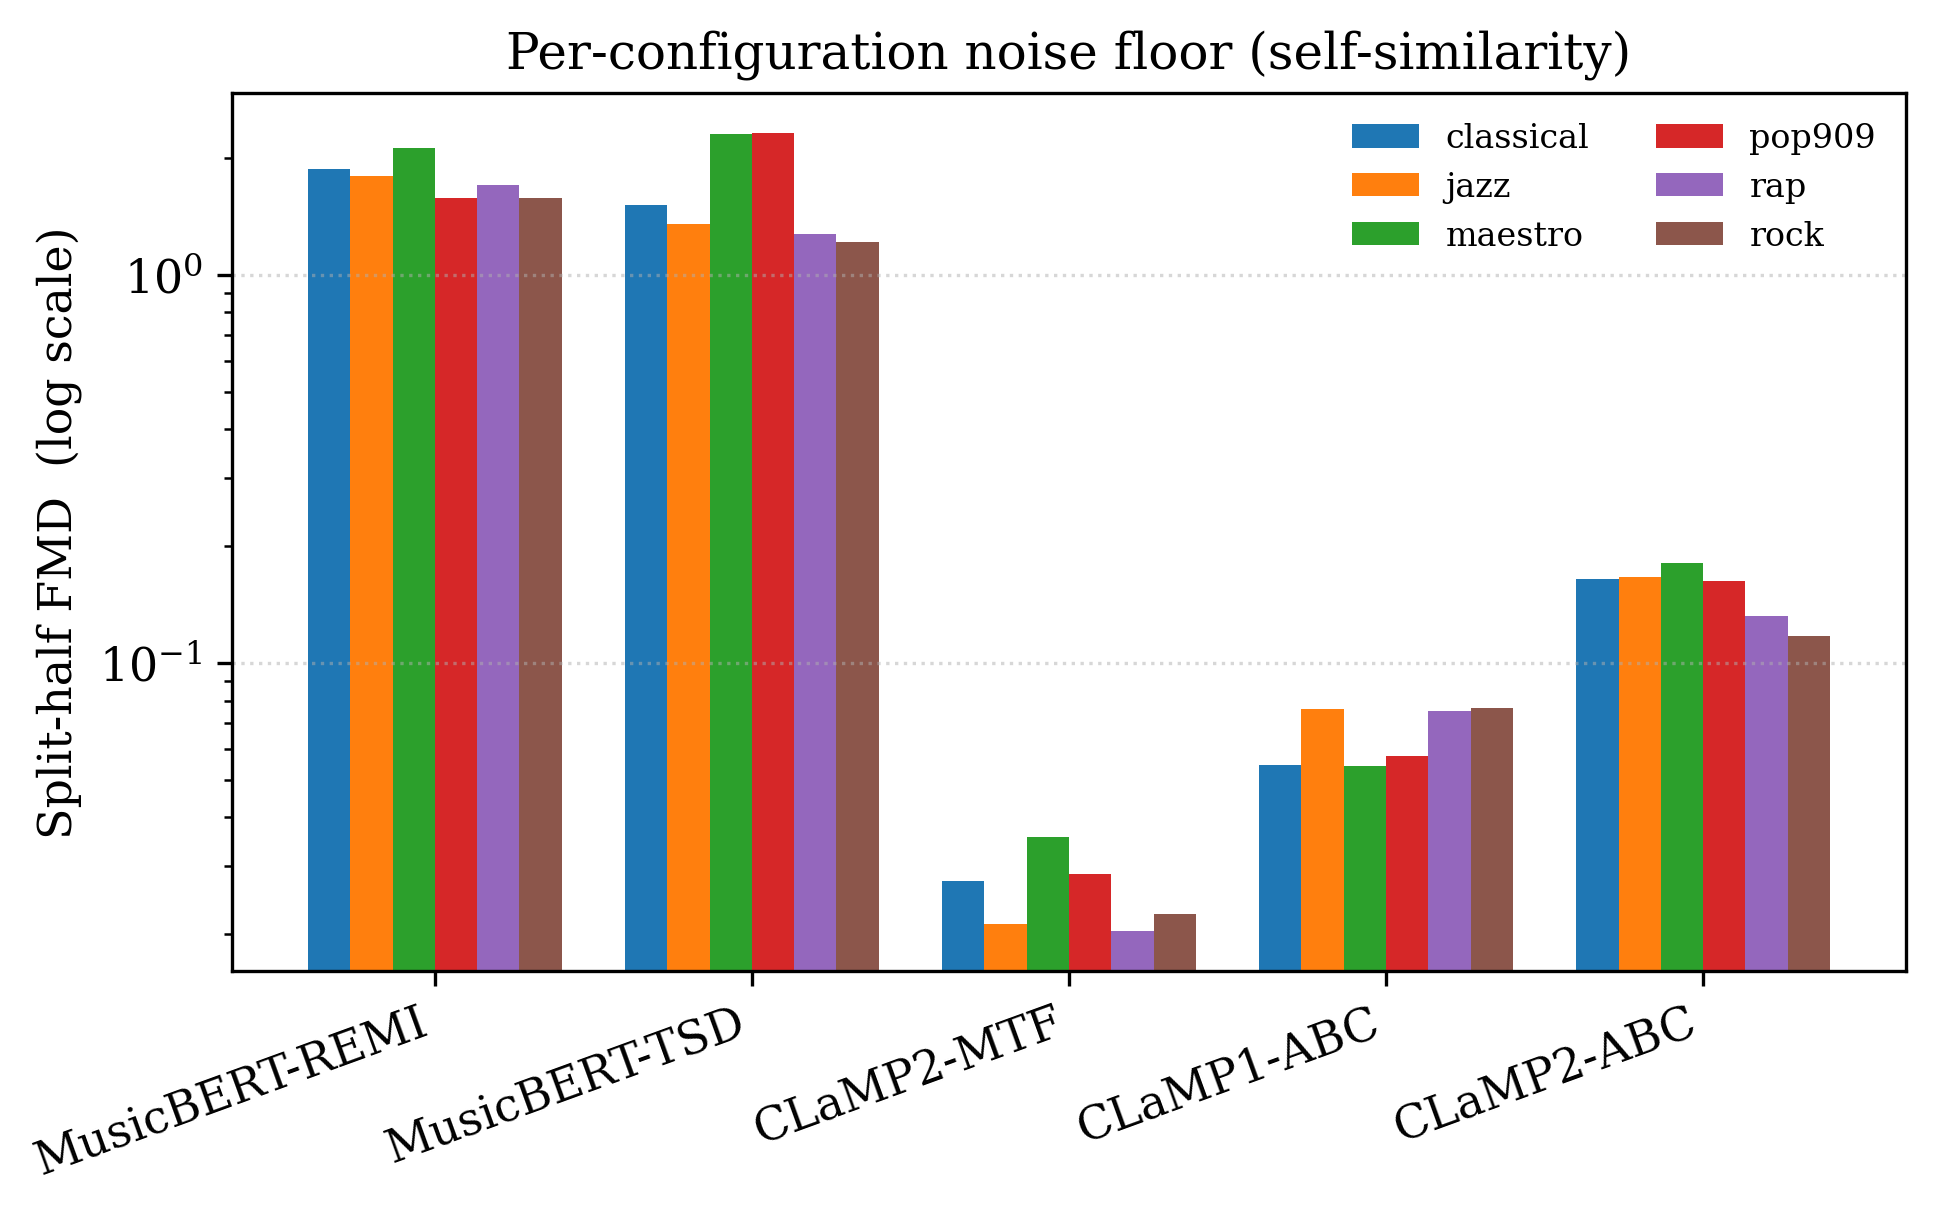
\includegraphics[width=0.92\linewidth]{fig1_noise_floor.png}
\caption{Per-configuration noise floor (split-half FMD), log scale. The
$\sim\!60\times$ CLaMP/MusicBERT separation reflects embedding geometry and
is divided out by the SNR of Eq.~\eqref{eq:snr}.}
\label{fig:floor}
\end{figure}

\subsection{Velocity is the only detected attribute --- and only where it is represented}
Table~\ref{tab:pert} gives the perturbation FMD, its SNR, bootstrap CI, and
permutation $p$ on MAESTRO; Table~\ref{tab:pertrep} replicates the study on
POP909. Figure~\ref{fig:snr} visualises the SNR and Figure~\ref{fig:forest}
the per-condition significance. Four points.

\textbf{(1)~Velocity.} Flattening velocity is the only perturbation whose
SNR exceeds $1$, and it is permutation-significant in exactly the three
representations that encode velocity --- \texttt{MusicBERT-REMI}
($\snr=3.16$, $p<0.01$), \texttt{MusicBERT-TSD} ($1.35$, $p<0.01$) and
\texttt{CLaMP2-MTF} ($1.18$, $p=0.02$). Under both ABC pipelines the
perturbed corpus renders to \emph{character-identical} ABC --- the
notation has no velocity channel --- so the embeddings are unchanged and
$\fmd=0.0000$ exactly. The blindness is structural, not statistical.

\textbf{(2)~The same-model control isolates the representation.} The
decisive comparison is within CLaMP-2: fed MTF, the model detects velocity
($\snr=1.18$, $p=0.02$); fed ABC --- with weights, architecture, and music
unchanged --- the response is exactly zero. Conversely, holding ABC fixed
and swapping the model (\texttt{CLaMP1-ABC} vs.\ \texttt{CLaMP2-ABC})
yields zero in both cases. The representation, not the model, gates what
the metric can detect.

\textbf{(3)~Microtiming and tempo.} $16$th-note quantization (SNR
$0.05$--$0.66$) and tempo flattening (SNR $0.04$--$0.20$) do not exceed
the noise floor for any configuration at $n=80$; even CLaMP-2/MTF, the
most timing-sensitive, does not cross the threshold. The \emph{combined}
perturbation (SNR up to $3.30$) simply tracks the velocity column ---
de-expression here is dominated by loss of dynamics.\footnote{The small
ABC responses to tempo flattening and the combined perturbation
($\snr\le0.41$, n.s.) come from the global tempo marking (\texttt{Q:}) in
the ABC header --- the one tempo-related token the notation does carry.}

\textbf{(4)~Tokenizer, and replication.} Holding MusicBERT fixed, REMI is
markedly more velocity-sensitive than TSD ($\snr=3.16$ vs.\ $1.35$): the
tokenizer alone reshapes the sensitivity profile. The POP909 replication
(Table~\ref{tab:pertrep}) reproduces the entire pattern, more strongly:
velocity is detected by all three velocity-bearing pipelines
($\snr=4.15$, $2.01$, $1.70$; all $p<0.01$) and produces exactly zero
under both ABC pipelines. The replication also passes a built-in sanity
check: POP909 is already grid-quantized, so the quantization perturbation
is a no-op there and FMD is exactly $0$ for the token pipelines ---
the protocol correctly reports nothing where nothing was changed.

\begin{table}[t]
\centering
\caption{Perturbation sensitivity on MAESTRO: raw FMD, SNR
(Eq.~\ref{eq:snr}), bootstrap $95\%$ CI, and permutation $p$. \textbf{Bold}
SNR marks a \emph{detected} attribute ($\snr\ge1$ and $p<0.05$). Generated
from \texttt{perturbation\_sensitivity.csv}.}
\label{tab:pert}
\small
\begin{tabular}{@{}llcccc@{}}
\toprule
Configuration & Perturbation & FMD & SNR & 95\% CI & perm.\ $p$ \\
\midrule
\texttt{MusicBERT-REMI} & Velocity removed & 7.3166 & \textbf{3.16} & [7.294,\,10.732] & $<$0.01 \\
\texttt{MusicBERT-REMI} & Timing quantized & 0.1043 & {0.05} & [0.730,\,2.217] & 1.00 \\
\texttt{MusicBERT-REMI} & Tempo flattened & 0.1483 & {0.06} & [0.755,\,1.825] & 1.00 \\
\texttt{MusicBERT-REMI} & All combined & 7.6272 & \textbf{3.30} & [7.528,\,9.427] & $<$0.01 \\
\addlinespace
\texttt{MusicBERT-TSD} & Velocity removed & 3.1343 & \textbf{1.35} & [3.387,\,5.348] & $<$0.01 \\
\texttt{MusicBERT-TSD} & Timing quantized & 0.2585 & {0.11} & [0.718,\,2.315] & 1.00 \\
\texttt{MusicBERT-TSD} & Tempo flattened & 0.3293 & {0.14} & [0.642,\,2.872] & 1.00 \\
\texttt{MusicBERT-TSD} & All combined & 3.9613 & \textbf{1.71} & [3.844,\,6.011] & $<$0.01 \\
\addlinespace
\texttt{CLaMP2-MTF} & Velocity removed & 0.0464 & \textbf{1.18} & [0.050,\,0.074] & 0.02 \\
\texttt{CLaMP2-MTF} & Timing quantized & 0.0259 & {0.66} & [0.034,\,0.055] & 0.08 \\
\texttt{CLaMP2-MTF} & Tempo flattened & 0.0050 & {0.13} & [0.013,\,0.030] & 1.00 \\
\texttt{CLaMP2-MTF} & All combined & 0.0608 & \textbf{1.55} & [0.065,\,0.087] & $<$0.01 \\
\addlinespace
\texttt{CLaMP1-ABC} & Velocity removed & 0.0000 & {0.00} & [0.017,\,0.036] & 1.00 \\
\texttt{CLaMP1-ABC} & Timing quantized & 0.0072 & {0.13} & [0.021,\,0.038] & 1.00 \\
\texttt{CLaMP1-ABC} & Tempo flattened & 0.0020 & {0.04} & [0.017,\,0.038] & 1.00 \\
\texttt{CLaMP1-ABC} & All combined & 0.0095 & {0.17} & [0.024,\,0.049] & 1.00 \\
\addlinespace
\texttt{CLaMP2-ABC} & Velocity removed & 0.0000 & {0.00} & [0.061,\,0.121] & 1.00 \\
\texttt{CLaMP2-ABC} & Timing quantized & 0.0438 & {0.22} & [0.094,\,0.168] & 1.00 \\
\texttt{CLaMP2-ABC} & Tempo flattened & 0.0393 & {0.20} & [0.083,\,0.153] & 1.00 \\
\texttt{CLaMP2-ABC} & All combined & 0.0823 & {0.41} & [0.114,\,0.195] & 0.97 \\
\bottomrule
\end{tabular}
\end{table}

\begin{table}[t]
\centering
\caption{Replication of the perturbation study on POP909. The full MAESTRO
pattern reproduces: velocity is detected only by velocity-bearing
representations; the quantization rows are an inherent sanity check (POP909
is already grid-quantized, so the perturbation is a no-op and FMD$=0$ for
the token pipelines). Generated from
\texttt{perturbation\_sensitivity\_pop909.csv}.}
\label{tab:pertrep}
\small
\begin{tabular}{@{}llcccc@{}}
\toprule
Configuration & Perturbation & FMD & SNR & 95\% CI & perm.\ $p$ \\
\midrule
\texttt{MusicBERT-REMI} & Velocity removed & 8.9865 & \textbf{4.15} & [8.880,\,11.435] & $<$0.01 \\
\texttt{MusicBERT-REMI} & Timing quantized & 0.0000 & {0.00} & [0.629,\,2.166] & 1.00 \\
\texttt{MusicBERT-REMI} & Tempo flattened & 0.0319 & {0.01} & [0.629,\,1.767] & 1.00 \\
\texttt{MusicBERT-REMI} & All combined & 9.1718 & \textbf{4.23} & [9.081,\,11.101] & $<$0.01 \\
\addlinespace
\texttt{MusicBERT-TSD} & Velocity removed & 3.9689 & \textbf{2.01} & [3.996,\,5.649] & $<$0.01 \\
\texttt{MusicBERT-TSD} & Timing quantized & 0.0000 & {0.00} & [0.540,\,1.681] & 1.00 \\
\texttt{MusicBERT-TSD} & Tempo flattened & 0.5583 & {0.28} & [0.808,\,2.442] & 0.98 \\
\texttt{MusicBERT-TSD} & All combined & 4.7993 & \textbf{2.43} & [4.535,\,6.457] & $<$0.01 \\
\addlinespace
\texttt{CLaMP2-MTF} & Velocity removed & 0.0638 & \textbf{1.70} & [0.065,\,0.093] & $<$0.01 \\
\texttt{CLaMP2-MTF} & Timing quantized & 0.0188 & {0.50} & [0.026,\,0.048] & 0.29 \\
\texttt{CLaMP2-MTF} & Tempo flattened & 0.0059 & {0.16} & [0.014,\,0.030] & 1.00 \\
\texttt{CLaMP2-MTF} & All combined & 0.0776 & \textbf{2.07} & [0.078,\,0.110] & $<$0.01 \\
\addlinespace
\texttt{CLaMP1-ABC} & Velocity removed & 0.0000 & {0.00} & [0.019,\,0.041] & 1.00 \\
\texttt{CLaMP1-ABC} & Timing quantized & 0.0000 & {0.00} & [0.019,\,0.038] & 1.00 \\
\texttt{CLaMP1-ABC} & Tempo flattened & 0.0014 & {0.02} & [0.019,\,0.039] & 1.00 \\
\texttt{CLaMP1-ABC} & All combined & 0.0014 & {0.02} & [0.021,\,0.039] & 1.00 \\
\addlinespace
\texttt{CLaMP2-ABC} & Velocity removed & 0.0000 & {0.00} & [0.050,\,0.119] & 1.00 \\
\texttt{CLaMP2-ABC} & Timing quantized & 0.0000 & {0.00} & [0.055,\,0.120] & 1.00 \\
\texttt{CLaMP2-ABC} & Tempo flattened & 0.0213 & {0.12} & [0.066,\,0.123] & 1.00 \\
\texttt{CLaMP2-ABC} & All combined & 0.0213 & {0.12} & [0.062,\,0.119] & 1.00 \\
\bottomrule
\end{tabular}
\end{table}

\begin{figure}[t]
\centering
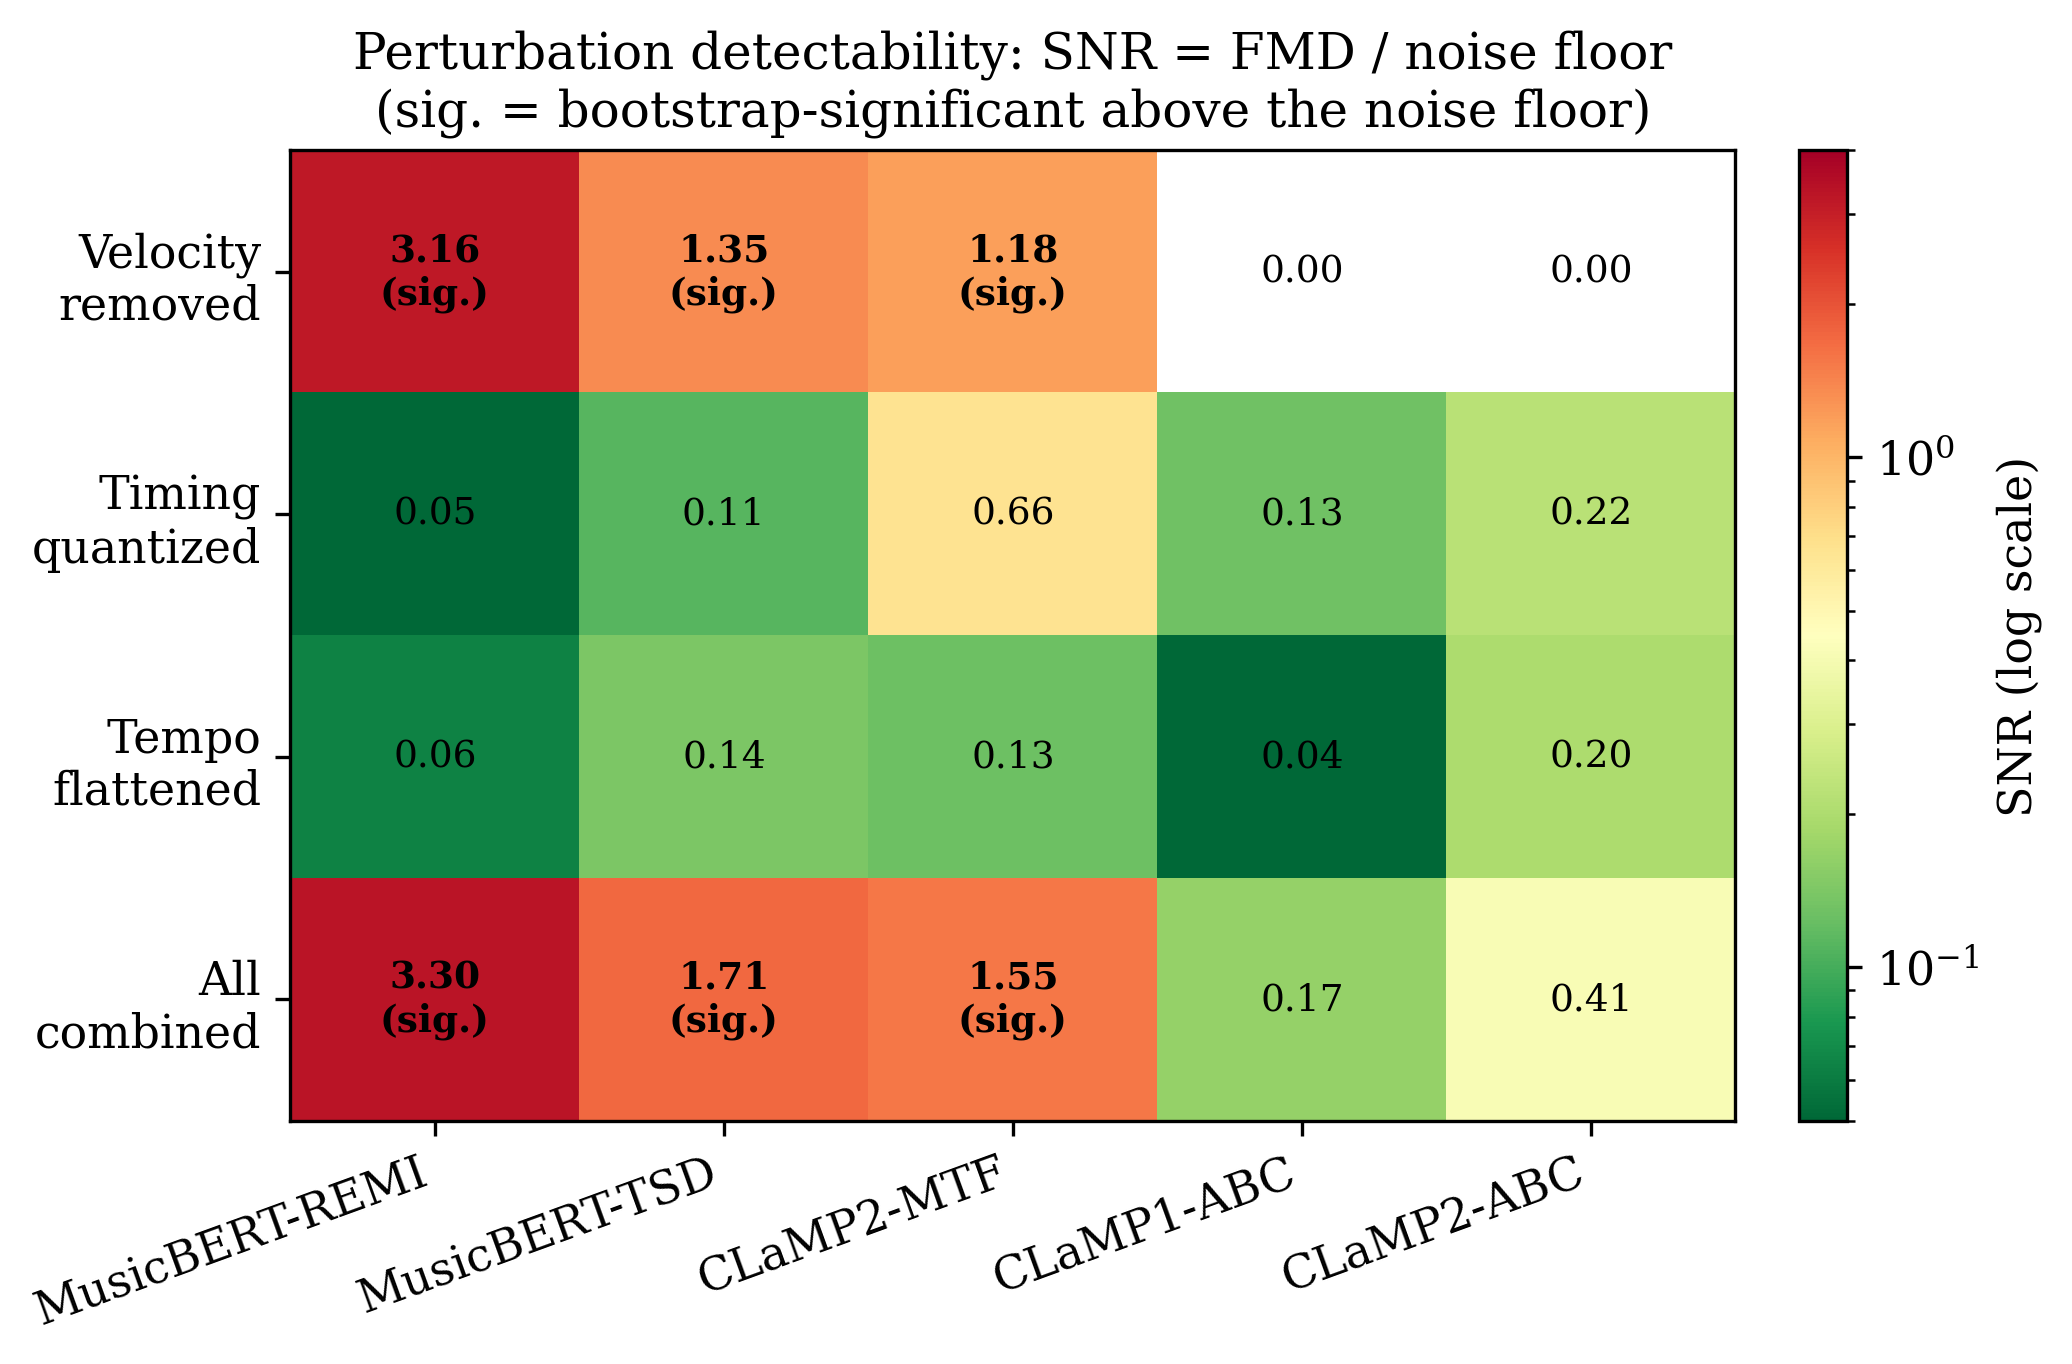
\includegraphics[width=\linewidth]{fig2_snr_heatmap.png}
\caption{Perturbation SNR. Velocity is detected by every velocity-bearing
representation but is invisible to ABC; timing and tempo are below the floor
everywhere.}
\label{fig:snr}
\end{figure}

\begin{figure}[t]
\centering
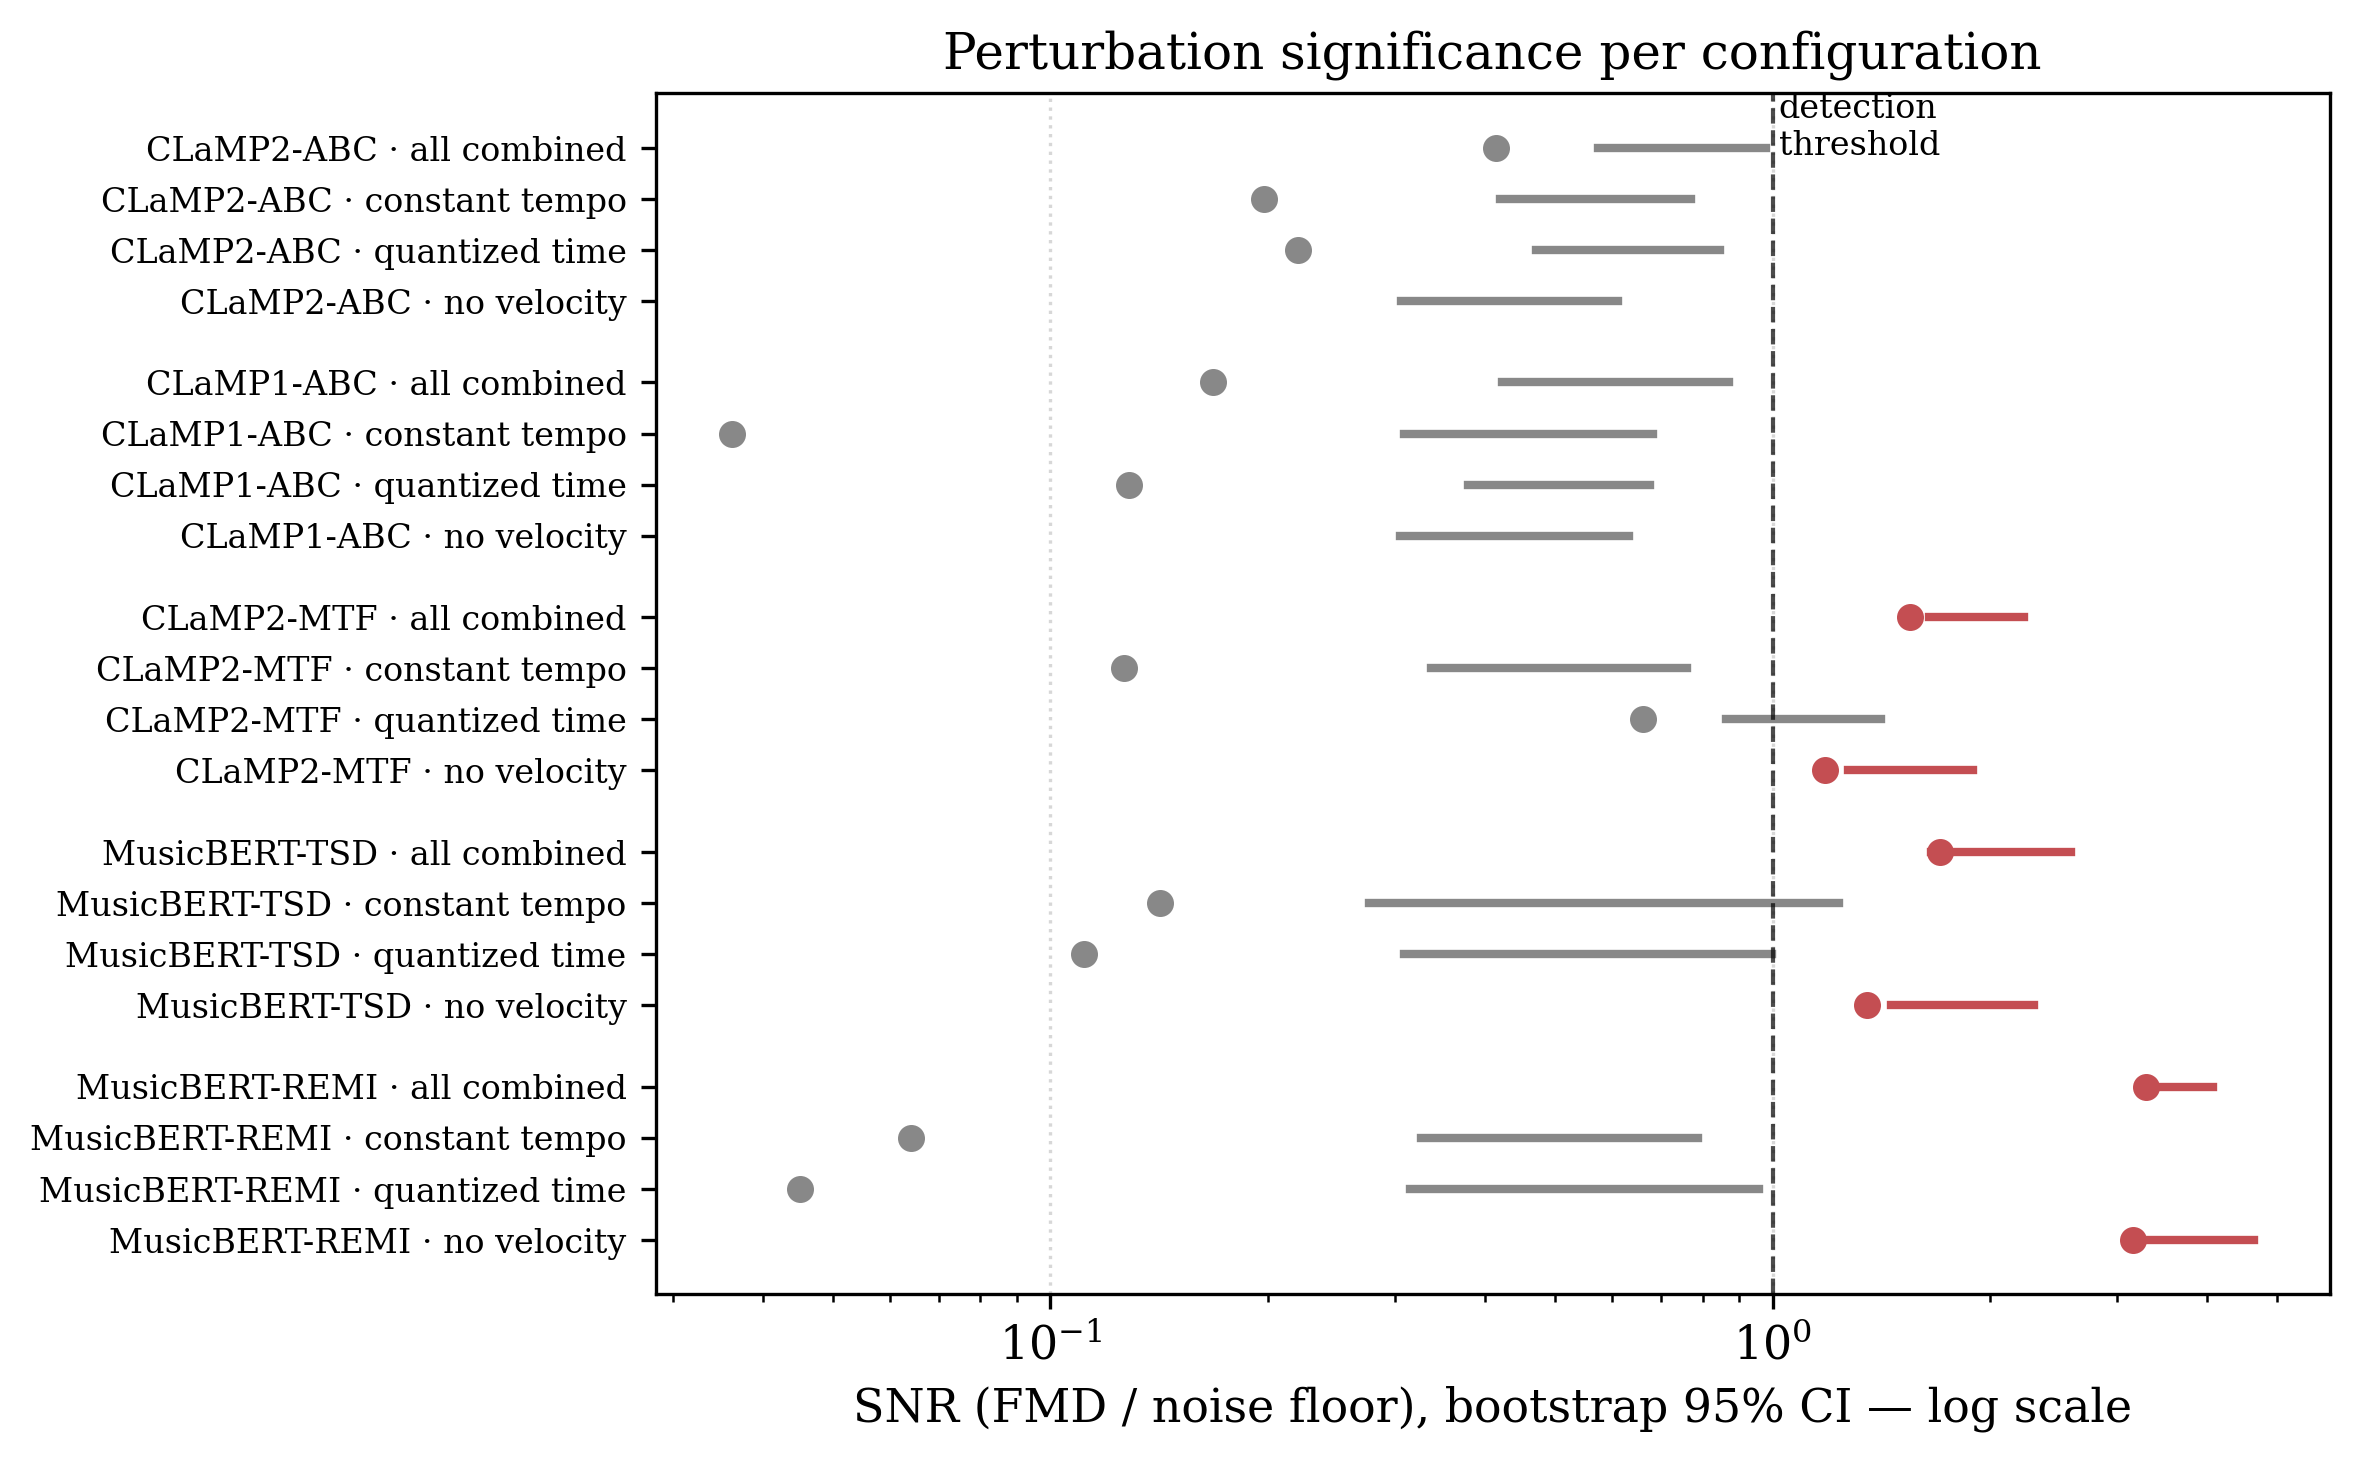
\includegraphics[width=0.95\linewidth]{fig4_perturbation_significance.png}
\caption{Per-condition SNR with bootstrap $95\%$ CI (log axis). The dashed
line is the detection threshold $\snr=1$; red marks permutation-significant
effects.}
\label{fig:forest}
\end{figure}

\subsection{The signal is file-level, not a distribution-fitting artifact}
Table~\ref{tab:paired} summarises the per-file paired analysis
(\S\ref{sec:method}). All five pipelines are deterministic, so the
per-file retest distance is exactly zero and any systematic shift is
attributable to the perturbation. Velocity flattening moves the embedding
of essentially \emph{every individual file} in the velocity-bearing
pipelines (Wilcoxon, Holm-adjusted $p\approx10^{-13}$ on both corpora),
while under both ABC pipelines the per-file shift is exactly zero for
every file. The same-model control contrast (velocity shift under MTF
vs.\ under ABC, within CLaMP-2's own embedding space) is significant at
$p_{\mathrm{Holm}}\approx10^{-13}$ on both corpora. The file-level view is
also \emph{more} sensitive than the distributional one: on MAESTRO,
quantization moves CLaMP-2/MTF embeddings of individual files reliably
($p_{\mathrm{Holm}}<10^{-12}$) even though the corpus-level effect stays
below the FMD detection floor ($\snr=0.66$) --- per-file shifts detect
attribute changes that corpus-level FMD cannot.

\begin{table}[t]
\centering
\caption{Per-file paired analysis, velocity flattening: median cosine
shift of a file's embedding and Holm-adjusted Wilcoxon $p$ (shift exceeds
the per-file re-encoding noise floor, which is $0$ for all pipelines).
Full per-cell results in \texttt{paired\_file\_tests*.csv}.}
\label{tab:paired}
\small
\begin{tabular}{@{}lcccc@{}}
\toprule
 & \multicolumn{2}{c}{MAESTRO} & \multicolumn{2}{c}{POP909} \\
Configuration & median shift & $p_{\mathrm{Holm}}$ & median shift & $p_{\mathrm{Holm}}$ \\
\midrule
\texttt{MusicBERT-REMI} & 0.0048 & $<10^{-12}$ & 0.0060 & $<10^{-12}$ \\
\texttt{MusicBERT-TSD}  & 0.0022 & $<10^{-12}$ & 0.0025 & $<10^{-12}$ \\
\texttt{CLaMP2-MTF}     & 0.0268 & $<10^{-12}$ & 0.0392 & $<10^{-12}$ \\
\texttt{CLaMP1-ABC}     & 0.0000 & 1.00 & 0.0000 & 1.00 \\
\texttt{CLaMP2-ABC}     & 0.0000 & 1.00 & 0.0000 & 1.00 \\
\addlinespace
control: MTF $>$ ABC (CLaMP-2) & \multicolumn{2}{c}{$p_{\mathrm{Holm}}<10^{-12}$} & \multicolumn{2}{c}{$p_{\mathrm{Holm}}<10^{-12}$} \\
\bottomrule
\end{tabular}
\end{table}

\subsection{Corpus-level rankings agree across pipelines}
Table~\ref{tab:spearman} and Figure~\ref{fig:spear} report the Spearman
rank agreement between configurations over the $15$ dataset pairs. Despite
their radically different attribute sensitivity, the five pipelines order
corpora largely alike: nine of ten configuration pairs agree significantly
($\rho=0.51$--$0.91$), with the strongest agreement between
\texttt{CLaMP2-MTF} and \texttt{CLaMP1-ABC} ($\rho=0.907$, $p<0.001$) ---
two pipelines in incomparable embedding spaces, one of which cannot see
dynamics at all. The only non-significant pair is REMI vs.\ TSD
($\rho=0.44$): the tokenizer perturbs the ranking more than the
model--representation change does. Read together with the perturbation
study, this resolves into a two-level picture: corpus-level stylistic
distances are carried by the pitch--rhythm core that every representation
shares, while expressive attributes (dynamics, microtiming) ride on top
and are visible only to representations that encode them. The separation
ratios (Table~\ref{tab:cross}) confirm that all five pipelines, including
both ABC ones, separate most genre pairs well above their own noise floors
(up to $4.8\times$).

\begin{table}[t]
\centering
\caption{Cross-configuration Spearman rank agreement over $15$ dataset
pairs (interpretable at $n\ge10$). \textbf{Bold} $\rho$ marks $p<0.05$.
Generated from \texttt{spearman\_ranking\_agreement.csv}.}
\label{tab:spearman}
\small
\begin{tabular}{@{}llccc@{}}
\toprule
Configuration A & Configuration B & $\rho$ & $p$ & $n$ \\
\midrule
\texttt{MusicBERT-REMI} & \texttt{MusicBERT-TSD} & 0.436 & 0.104 & 15 \\
\texttt{MusicBERT-REMI} & \texttt{CLaMP2-MTF} & \textbf{0.825} & $<$0.001 & 15 \\
\texttt{MusicBERT-REMI} & \texttt{CLaMP1-ABC} & \textbf{0.868} & $<$0.001 & 15 \\
\texttt{MusicBERT-REMI} & \texttt{CLaMP2-ABC} & \textbf{0.811} & $<$0.001 & 15 \\
\texttt{MusicBERT-TSD} & \texttt{CLaMP2-MTF} & \textbf{0.525} & 0.044 & 15 \\
\texttt{MusicBERT-TSD} & \texttt{CLaMP1-ABC} & \textbf{0.621} & 0.013 & 15 \\
\texttt{MusicBERT-TSD} & \texttt{CLaMP2-ABC} & \textbf{0.514} & 0.050 & 15 \\
\texttt{CLaMP2-MTF} & \texttt{CLaMP1-ABC} & \textbf{0.907} & $<$0.001 & 15 \\
\texttt{CLaMP2-MTF} & \texttt{CLaMP2-ABC} & \textbf{0.836} & $<$0.001 & 15 \\
\texttt{CLaMP1-ABC} & \texttt{CLaMP2-ABC} & \textbf{0.907} & $<$0.001 & 15 \\
\bottomrule
\end{tabular}
\end{table}

\begin{figure}[t]
\centering
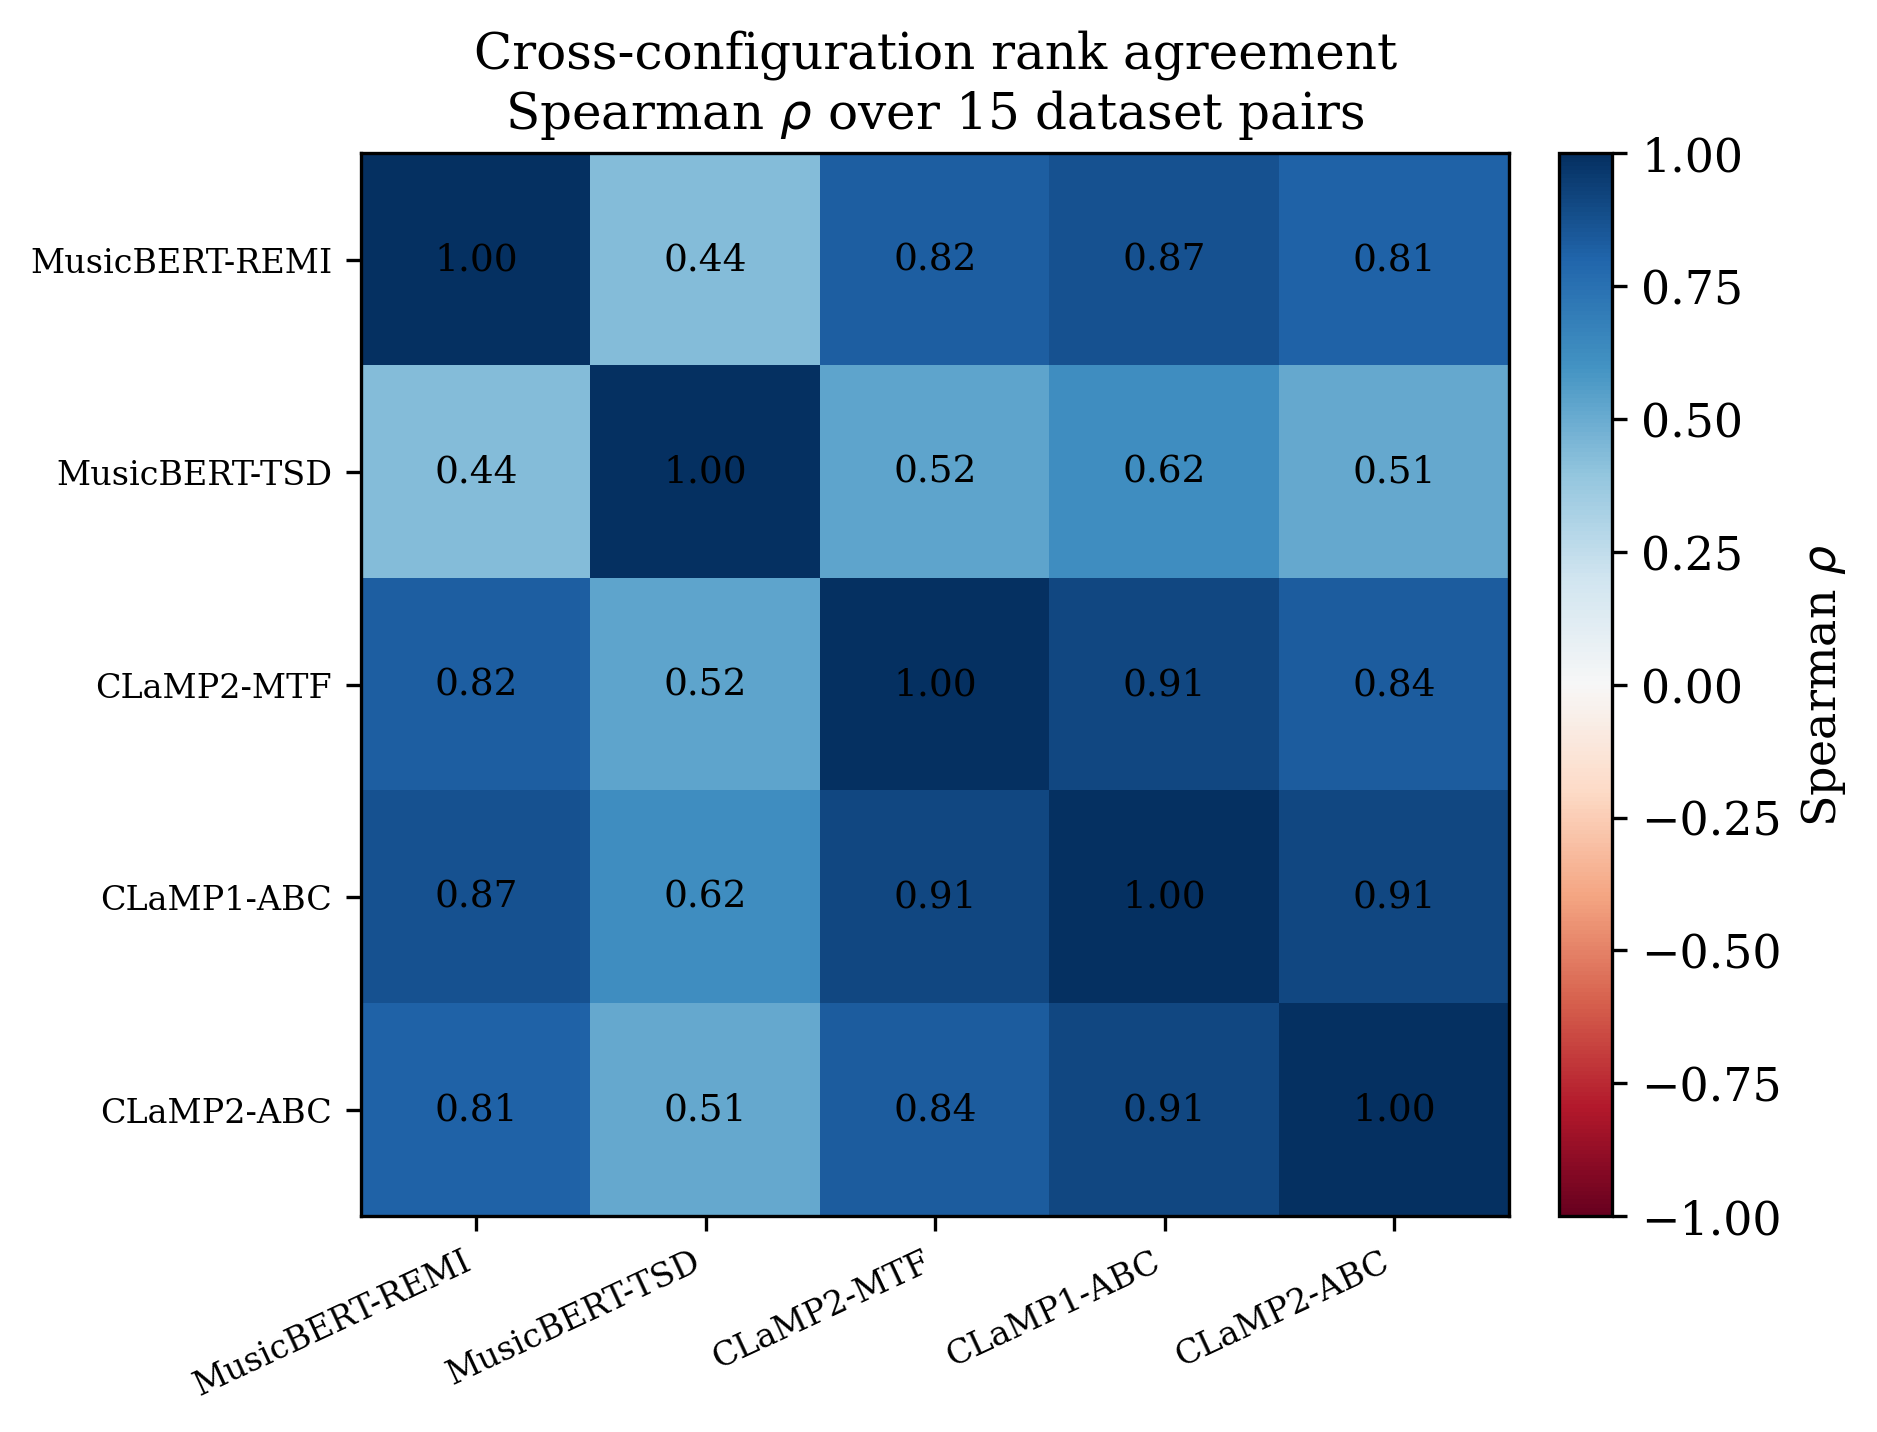
\includegraphics[width=0.72\linewidth]{fig5_spearman_heatmap.png}
\caption{Cross-configuration rank agreement (Spearman $\rho$, $n=15$).
Nine of ten pairs agree significantly; only REMI vs.\ TSD does not.}
\label{fig:spear}
\end{figure}

\begin{table}[t]
\centering
\caption{Cross-dataset separation ratio (FMD normalised by each
configuration's noise floor; $>1$ = above sampling noise), so values are
comparable across configurations. Generated from \texttt{cross\_dataset\_fmd.csv}.}
\label{tab:cross}
\small
\begin{tabular}{@{}lccccc@{}}
\toprule
Dataset pair & MusicBERT-REMI & MusicBERT-TSD & CLaMP2-MTF & CLaMP1-ABC & CLaMP2-ABC \\
\midrule
maestro\_vs\_rock & 2.83 & 2.88 & 3.12 & 2.29 & 3.85 \\
maestro\_vs\_rap & 2.49 & 6.85 & 3.72 & 3.35 & 4.80 \\
maestro\_vs\_jazz & 2.36 & 4.00 & 2.66 & 1.89 & 2.42 \\
classical\_vs\_rap & 2.21 & 6.64 & 3.18 & 3.21 & 4.65 \\
classical\_vs\_rock & 2.18 & 1.88 & 2.52 & 2.16 & 3.73 \\
pop909\_vs\_jazz & 2.06 & 3.98 & 1.92 & 1.40 & 1.70 \\
pop909\_vs\_rock & 1.96 & 1.89 & 2.04 & 1.76 & 2.67 \\
pop909\_vs\_rap & 1.92 & 6.63 & 2.88 & 2.78 & 3.80 \\
jazz\_vs\_rap & 1.84 & 4.41 & 1.67 & 1.51 & 3.48 \\
classical\_vs\_jazz & 1.81 & 3.67 & 2.11 & 1.62 & 2.26 \\
jazz\_vs\_rock & 1.78 & 3.41 & 2.04 & 1.00 & 2.57 \\
maestro\_vs\_pop909 & 1.65 & 1.94 & 1.35 & 0.73 & 1.47 \\
rock\_vs\_rap & 1.60 & 4.62 & 1.69 & 1.06 & 1.25 \\
pop909\_vs\_classical & 1.57 & 1.47 & 1.86 & 0.67 & 1.43 \\
maestro\_vs\_classical & 1.36 & 1.41 & 1.29 & 0.60 & 0.89 \\
\bottomrule
\end{tabular}
\end{table}

\subsection{Bootstrap stability}
Table~\ref{tab:boot} reports the bootstrap of the MAESTRO--POP909 distance.
Read through the scale-invariant CV, the configurations are comparably
stable ($8$--$20\%$), with \texttt{MusicBERT-TSD} the most variable. We do
\emph{not} compare the mean columns across the CLaMP/MusicBERT boundary:
those magnitudes live in incomparable spaces.

\begin{table}[t]
\centering
\caption{Bootstrap stability of the MAESTRO--POP909 FMD ($50$ resamples,
$N=80$). CV is scale-invariant and comparable across configurations; the
mean and CI are not. Generated from \texttt{bootstrap\_stability.csv}.}
\label{tab:boot}
\small
\begin{tabular}{@{}lcccc@{}}
\toprule
Configuration & mean & std & 95\% CI & CV \\
\midrule
\texttt{MusicBERT-REMI} & 3.5110 & 0.5314 & [2.662,\,4.637] & 15.1\% \\
\texttt{MusicBERT-TSD} & 3.9238 & 0.7910 & [2.742,\,5.473] & 20.2\% \\
\texttt{CLaMP2-MTF} & 0.0478 & 0.0067 & [0.039,\,0.060] & 14.0\% \\
\texttt{CLaMP1-ABC} & 0.0683 & 0.0054 & [0.059,\,0.080] & 8.0\% \\
\texttt{CLaMP2-ABC} & 0.2769 & 0.0221 & [0.243,\,0.320] & 8.0\% \\
\bottomrule
\end{tabular}
\end{table}

% =====================================================================
\section{Discussion}
\label{sec:discussion}
% =====================================================================
\paragraph{What an FMD score actually measures.}
The results support a two-level picture. At the \emph{attribute} level the
input representation sets a hard ceiling on detectability --- an attribute
the representation discards (velocity under ABC) is invisible no matter
how good the model is --- and within that ceiling the model and tokenizer
modulate how strongly the surviving attributes register. The same-model
control makes this causal rather than correlational: with weights and data
held fixed, switching CLaMP-2 from MTF to ABC turns the velocity response
off exactly. At the \emph{corpus} level, however, stylistic rankings agree
broadly across all five pipelines ($\rho$ up to $0.907$ between MTF and
ABC): genre distances are carried by the pitch--rhythm core that every
representation shares, so a pipeline can rank corpora ``correctly'' while
being entirely blind to the expressive attributes a practitioner may care
about. Practically, ``does my FMD rank styles sensibly?'' and ``does my
FMD see dynamics?'' are different questions with different answers, and
only a perturbation audit distinguishes them.

\paragraph{A negative result worth stating.}
Earlier analyses of this data reported, for example, that one model was
``$63\times$ more consistent'' or ``$730\times$ more expressive'' than
another. Such statements divide raw FMD across the normalisation boundary
and are scale artifacts: $L_2$ normalisation shrinks every distance CLaMP
produces and the lack of it inflates every distance MusicBERT produces,
independent of musical content. The honest, comparable statements are the
SNR-, permutation-, and rank-based ones above. We highlight this because the
same trap awaits anyone benchmarking generative systems with FMD scores
computed from different backbones.

\paragraph{Practitioner guidance.}
\emph{(i)}~Match the representation to the attribute under study: to
evaluate dynamics use a velocity-bearing representation (REMI/TSD tokens or
MTF), never ABC; ABC is appropriate for score-like stylistic comparison ---
it ranks corpora consistently with the other pipelines while being
invariant to performance nuance by construction.
\emph{(ii)}~Never compare raw FMD across embedding models; if a cross-model
statement is unavoidable, use SNR, Spearman, or CV. \emph{(iii)}~Treat
microtiming/tempo FMD with suspicion at small $n$: neither cleared the
corpus-level detection floor in any configuration here (though per-file
shifts can still be demonstrated for MTF). \emph{(iv)}~Audit the input
conversion: a per-file retest (encode the same unperturbed file twice) is
nearly free and immediately exposes nondeterministic or broken rendering
--- it is how a silent conversion failure was caught in this study.

% =====================================================================
\section{Limitations and Threats to Validity}
\label{sec:limitations}
% =====================================================================
\begin{itemize}\itemsep2pt
\item \textbf{MusicBERT input rendering.} Our MusicBERT pipelines encode
MidiTok token \emph{identifiers} as text via the model's subword tokenizer
rather than the native OctupleMIDI encoding; this likely contributes to
MusicBERT's high, unnormalised noise floor and should be read as a
tokenization-sensitivity baseline, not as MusicBERT used canonically.
\item \textbf{Sample size vs.\ dimension.} With $n=40$--$80$ samples and
$d=768$ dimensions, the covariance in Equation~\eqref{eq:fmd} is
rank-deficient and ridge-regularised; absolute FMD magnitudes (especially
for unnormalised embeddings) are biased upward. The SNR, permutation, and CV
framings mitigate but do not remove this; larger $n$ would tighten every
estimate.
\item \textbf{ABC rendering granularity.} Our ABC renderer quantizes to a
sixteenth-note grid and reduces dense polyphony to chorded onsets. This
reflects the score-like nature of ABC (performance nuance is discarded by
design), but it also means sub-sixteenth detail is invisible to the ABC
pipelines by construction, independent of the embedding model.
\item \textbf{One strength per attribute.} Each attribute is ablated at a
single perturbation strength (e.g.\ one quantization grid); a
dose--response sweep would turn the binary detected/undetected verdict
into detection thresholds.
\item \textbf{Genre-subset provenance.} The four genre datasets are
Lakh-derived; instrument normalisation mitigates but does not eliminate
provenance confounds in the cross-dataset ranking.
\end{itemize}

% =====================================================================
\section{Conclusion}
% =====================================================================
We profiled five Fr\'echet Music Distance pipelines by perturbing musically
interpretable attributes, by a per-file paired analysis with a re-encoding
noise floor, and by comparing cross-dataset rankings --- using only
scale-invariant statistics because raw FMD is not comparable across
embedding spaces, a point we both explain and demonstrate. At the
attribute level the input representation is decisive: velocity is detected
only where it is represented (SNR up to $4.2$ across two corpora,
per-file $p\approx10^{-13}$), is \emph{exactly} invisible under ABC, and
the same-model control shows the response switching off when only the
representation changes; microtiming and tempo stay below the corpus-level
detection floor everywhere. At the corpus level, by contrast, all five
pipelines rank styles largely alike ($\rho$ up to $0.907$): ranking
sanity does not certify attribute sensitivity. We recommend reporting FMD
\emph{sensitivity}, not just FMD, and provide a small, reusable, fully
scripted protocol for doing so.

% =====================================================================
\section*{Reproducibility}
% =====================================================================
All numbers derive from
\texttt{results/reports/sensitivity\_pivot/} (CSV/JSON), produced by
\texttt{python main.py --mode sensitivity}. Every table and figure in this
paper was generated programmatically from those CSVs by
\texttt{scripts/generate\_draft\_tables.py} and
\texttt{scripts/generate\_draft\_figures.py} (no result was transcribed by
hand). Configurations, datasets, perturbations, and seeds are fixed in
\texttt{configs/sensitivity\_pivot.yaml}; the code is available at
\texttt{github.com/Michal2390/FMD-sensitivity-for-tokenization-and-embeddings}.

% =====================================================================
\begin{thebibliography}{99}
\small

\bibitem{retkowski2025fmd}
J.~Retkowski, J.~St\k{e}pniak, and M.~Modrzejewski,
``Fr\'echet Music Distance: A Metric for Generative Symbolic Music
Evaluation,'' 2025. Code: \texttt{github.com/jryban/frechet-music-distance}.

\bibitem{heusel2017fid}
M.~Heusel, H.~Ramsauer, T.~Unterthiner, B.~Nessler, and S.~Hochreiter,
``GANs Trained by a Two Time-Scale Update Rule Converge to a Local Nash
Equilibrium,'' in \emph{NeurIPS}, 2017.

\bibitem{kilgour2019fad}
K.~Kilgour, M.~Zuluaga, D.~Roblek, and M.~Sharifi,
``Fr\'echet Audio Distance: A Reference-Free Metric for Evaluating Music
Enhancement Algorithms,'' in \emph{Interspeech}, 2019.

\bibitem{dowson1982frechet}
D.~C.~Dowson and B.~V.~Landau,
``The Fr\'echet Distance between Multivariate Normal Distributions,''
\emph{Journal of Multivariate Analysis}, vol.~12, no.~3, 1982.

\bibitem{zeng2021musicbert}
M.~Zeng, X.~Tan, R.~Wang, Z.~Ju, T.~Qin, and T.-Y.~Liu,
``MusicBERT: Symbolic Music Understanding with Large-Scale Pre-Training,''
in \emph{Findings of ACL-IJCNLP}, 2021.

\bibitem{wu2023clamp}
S.~Wu, D.~Yu, X.~Tan, and M.~Sun,
``CLaMP: Contrastive Language--Music Pre-training for Cross-Modal Symbolic
Music Information Retrieval,'' in \emph{ISMIR}, 2023.

\bibitem{wu2024clamp2}
S.~Wu et al.,
``CLaMP~2: Multimodal Music Information Retrieval Across 101 Languages Using
Large Language Models,'' 2024.

\bibitem{fradet2021miditok}
N.~Fradet, J.-P.~Briot, F.~Chhel, A.~El~Fallah~Seghrouchni, and
N.~Gutowski,
``MidiTok: A Python Package for MIDI File Tokenization,'' in
\emph{ISMIR Late-Breaking Demo}, 2021. Code:
\texttt{github.com/Natooz/MidiTok}.

\bibitem{huang2020remi}
Y.-S.~Huang and Y.-H.~Yang,
``Pop Music Transformer: Beat-Based Modeling and Generation of Expressive
Pop Piano Compositions'' (REMI), in \emph{ACM Multimedia}, 2020.

\bibitem{hawthorne2019maestro}
C.~Hawthorne et al.,
``Enabling Factorized Piano Music Modeling and Generation with the MAESTRO
Dataset,'' in \emph{ICLR}, 2019.

\bibitem{wang2020pop909}
Z.~Wang et al.,
``POP909: A Pop-Song Dataset for Music Arrangement Generation,'' in
\emph{ISMIR}, 2020.

\bibitem{le2024nlpsurvey}
D.~V.~T.~Le, L.~Bigo, M.~Keller, and D.~Herremans,
``Natural Language Processing Methods for Symbolic Music Generation and
Information Retrieval: a Survey,'' \emph{arXiv:2402.17467}, 2024.

\end{thebibliography}

\end{document}
